% 
% Annual Cognitive Science Conference
% Sample LaTeX Paper -- Proceedings Format
% 

% Original : Ashwin Ram (ashwin@cc.gatech.edu)       04/01/1994
% Modified : Johanna Moore (jmoore@cs.pitt.edu)      03/17/1995
% Modified : David Noelle (noelle@ucsd.edu)          03/15/1996
% Modified : Pat Langley (langley@cs.stanford.edu)   01/26/1997
% Latex2e corrections by Ramin Charles Nakisa        01/28/1997 
% Modified : Tina Eliassi-Rad (eliassi@cs.wisc.edu)  01/31/1998
% Modified : Trisha Yannuzzi (trisha@ircs.upenn.edu) 12/28/1999 (in process)
% Modified : Mary Ellen Foster (M.E.Foster@ed.ac.uk) 12/11/2000
% Modified : Ken Forbus                              01/23/2004
% Modified : Eli M. Silk (esilk@pitt.edu)            05/24/2005
% Modified: Niels Taatgen (taatgen@cmu.edu)  10/24/2006

%% Change ``a4paper'' in the following line to ``letterpaper'' if you are
%% producing a letter-format document.

\documentclass[10pt,letterpaper]{article}

\usepackage{cogsci}
\usepackage{pslatex}
\usepackage{apacite}

\usepackage{amsmath}
\usepackage{mathrsfs}
\usepackage{graphicx}
%\usepackage{amsthm}


%% These are for sub-numbering hypotheses. E.g. Hyp1A, Hyp1B
\usepackage{ntheorem}

\newtheorem{Definition}{Definition}
\newtheorem{hyp}{Hypothesis}

\makeatletter
\newcounter{subhyp} 
\let\savedc@hyp\c@hyp
\newenvironment{subhyp}
 {%
  \setcounter{subhyp}{0}%
  \stepcounter{hyp}%
  \edef\saved@hyp{\thehyp}% Save the current value of hyp
  \let\c@hyp\c@subhyp     % Now hyp is subhyp
  \renewcommand{\thehyp}{\saved@hyp\alph{hyp}}%
 }
 {}
\newcommand{\normhyp}{%
  \let\c@hyp\savedc@hyp % revert to the old one
  \renewcommand\thehyp{\arabic{hyp}}%
} 
\makeatother
%% End sub numbering hypotheses


\title{ A relational lay theory of emotion: \\ Making and integrating multiple emotion attributions }
 
\author{{\large \bf Desmond C. Ong}, 
{\large \bf Jamil Zaki}, 
{\large \bf Noah D. Goodman} \\
\texttt{\{dco, jzaki, ngoodman\}@stanford.edu} \\
  Department of Psychology, Stanford University, Stanford CA, USA 
}



\begin{document}

\maketitle

\begin{abstract}
abstract text

\textbf{Keywords:} 
Affective cognition; Emotions; Social cognition; Computational Modeling
\end{abstract}

Intro

%you could say that there's simple ``bob feels E" and relational ``bob feels E about X" type emotion attributions, where E is an emotion and X is an event. there are two questions to address: what is the relation between the two types of attribution, and what is the relation between two relational ones, depending on the relation between the events.


%In our daily lives, we constantly interact with others around us, and invariably have to reason about others' emotional states. 
%
%
%There are two classes of intuitive attributions than observers often make, the first being simple emotional state attributions -- ``Bob feels happy (in general)". Some affective scientists might point out that in the absence of  The second class of emotional state attributions are relational in nature: ``Bob feels happy about X", where X can be an event like ``receiving a promotion" or ``seeing his children". 
%
%	Relational attributions are justifiable according to some lay causal theory. Intuitively, emotions must be ``caused" by some event in the world, and 
%
%
%Observers have a lay theory that something Lay observers often attribute emotions 
%	Indeed, affective and cognitive scientists have debated for decades over whether 


%How does an observer infer that agents (the targets of affective cognition) who spill a cup of coffee, miss the bus, or fall off a bicycle, likely feel similar emotions, such as sadness? One problem that any model of affective cognition must deal with is the combinatorial explosion of outcomes and emotional states that people can experience. It would be both inefficient and impractical for observers to store or retrieve knowledge about the likely affective consequences of every possible situation. We hypothesize that people circumvent this complexity by evaluating situations based on a smaller number of �active psychological ingredients� those situations contain. For instance, many emotion-inducing situations share key common features (e.g., the attainment or nonattainment of goals) that consistently produce particular emotions (Barrett, Mesquita, Ochsner, & Gross, 2007; Ellsworth & Scherer, 2003). An individual in a situation can take advantage of this commonality by appraising the situation along a small number of relevant appraisal dimensions: that is, reducing a situation to a low-dimensional set of emotion-relevant features (Ortony, Clore, & Collins, 1988; Schachter & Singer, 1962; Scherer, Schorr, & Johnstone, 2001; Smith & Lazarus, 1993). 



\subsection{Making multiple relational attributions}

What is the relation between two relational attributions? 

\begin{Definition}
Relational Emotion Attribution is a function $E_R$ that takes the agent $A$ and the event $X$, and returns real-valued numbers corresponding to the intensity of $A$'s emotions. $E_R(A,X)$ returns the emotions attributed to agent $A$ following event $X$.
\end{Definition}

\begin{subhyp}
\begin{hyp} \label{Hypothesis:NoCrossTalk}
\textbf{Independence.} Following events X and Y, the emotions attributed to each event would be independent of the features of the other event. That is, $E_R(A,X)$ does not depend on the features of $Y$, and vice versa.
\end{hyp}

\begin{hyp} \label{Hypothesis:CrossTalk}
\textbf{No Independence.} Following events X and Y, the emotions attributed to each event would be dependent of the features of the other event. That is, $E_R(A,X)$ would depend on the features of $Y$, and vice versa.
\end{hyp}
\end{subhyp}

\subsection{Integrating to give simple emotion attributions}
What is the relation between relational and simple emotion attribution?
\begin{Definition}
Simple Emotion Attribution is a function $E_S$ that takes only the agent $A$ and returns real-valued numbers corresponding to the intensity of $A$'s emotions. $E_S(A)$ returns the current emotions attributed to agent $A$.
\end{Definition}


%H1: Mood = average
%H2: Mood = time-weighted average (more recent events matter more)

\begin{subhyp}
\begin{hyp} \label{Hypothesis:SimpleAverage}
\textbf{Simple Average.} Following events X and Y, the overall emotion would be a simple average of the two relational attributions, i.e. $E_S(A) = b_0 + b_1 [E_R(A,X) + E_R(A,Y) ]$.
\end{hyp}

\begin{hyp} \label{Hypothesis:RecencyWeighted}
\textbf{Recency-Weighted Average.} Following events X and Y, the overall emotion would be a recency-weighted average of the two relational attributions, i.e. $E_S(A) = b_0 + b_1 E_R(A,X) + b_2 E_R(A,Y)$, and $b_2>b_1$ iff $Y$ occurred later than $X$.
\end{hyp}
\end{subhyp}



\section{Results:}

\begin{itemize}
\item No Crosstalk: Ps can separate emotions attributed to event X and Y. i.e. $E_R(A,X)$ is independent of $Y$.
\item Effect of expectations. Even though there's no cross-talk, the mere existence of the second event affects the features of X (removes loss aversion). The existence of $Y$ qualitatively changes $\mathscr{F}(X)$.
\item No Loss Aversion. In judging emotions across multiple events, people expect no loss aversion.
\item Temporal order matters. Participants' lay theories are sensitive to the temporal ordering of events: if $X$ happened, then $Y$ happened, $Y$ matters more to overall emotion $E_S(A)$. Agent-recency.
\item Evidence presentation order matters (observer-recency effect). The order in which participants make attributions also affects: if they first make an attribution to a temporally later event $Y$ then to a temporally earlier event $X$, their judgments about overall emotion $E_S(A)$ would not favor the later event $Y$. The attribution that the participant most recently gave is weighed more.

\end{itemize}



%do a multilevel analysis to see if maybe some participants are sensitive to both; some are not.? maybe accounted for 
%
%
%relate context
%with elemental relational attributions
%and overall mood attributions
%
%revisit analysis based on hypotheses of these components
%
%look at a "first-half, last-half" analysis. It's a somewhat hard experiment, maybe Ss are getting tired or bored.
%
%sanity check: how much did he win overall?
%
%---
%
%recency: maybe show decay?
%
%8am vs noon
%10am vs noon
%
%crossed with
%
%ask about mood at 2pm
%ask about mood at 4pm
%        
%----





\section{Behavioral Experiments}

\subsection{Basic Paradigm Description}
The basic experimental paradigm across all experiments described in this paper involves watching a character play a spinning wheel. The characters spun wheels and ostensibly won an amount of money depending on where each wheel landed (Fig. \ref{ParadigmFig}). Each wheel comprised three possible outcomes, all of which were non-negative. We systematically de-correlated the probabilities of the outcomes and the values of the outcomes of each wheel, such that the reward amount and expected values are de-correlated. 

% XXX TODO fix this citation
In our previous work (Ong, Zaki, \& Goodman, under review), we analyzed how the parameters of a single situation $X$ affect participant judgments of emotions to an agent $A$, or $E_R(A,X)$. That is, what are the features of the situation $X$, $\mathscr{F}(X)$, that reliably predict $E_R(A,X)$. We identified three predictors that consistently and significantly predicted all the emotions we measured: the amount won (win($X$)), the prediction error (PE($X$) = amount won - expected value of $X$), and the absolute value of the prediction error (absPE($X$)). The first two are naturally predicted from standard utility theory. The third predictor indicates that participants' sensitivity to negative prediction errors were stronger than to positive prediction errors, indicating a measurable indicator of \textit{loss aversion} (cites).\footnote{The PE, absPE formulation is mathematically equivalent to the more common, piecewise formulation of loss aversion: $y=a PE, PE \geq 0$ and $y=b PE, PE < 0$. In our model, we require just one equation across the whole domain, $y=c PE + d |PE|$. We can easily show that $a = c + d$, and $b = c - d$.} Using the formulation we had above, we built a regression model to predict emotion attribution following an event $X$: 
\begin{align}
E_R(A,X) &= E_R(A,\mathscr{F}(X)) \\
&= b_0 + b_1 \text{win}(X) + b_2 \text{PE}(X) + b_3 \text{absPE}(X) + \epsilon  \nonumber
\end{align}
Thus, we had a predefined analysis plan for analyzing the experiments in this paper.



\subsection{Experiment 1}
In Experiment 1, participants made attributions of emotion to a character following two separate events, followed by an overall attribution.

\subsubsection{Participants.} We recruited 150 participants through Amazon's Mechanical Turk and paid them for completing the experiment. All experiments reported in this paper were conducted according to guidelines approved by the Institutional Review Board at Stanford University.

\subsubsection{Procedures.} 


\begin{figure}[htb!]
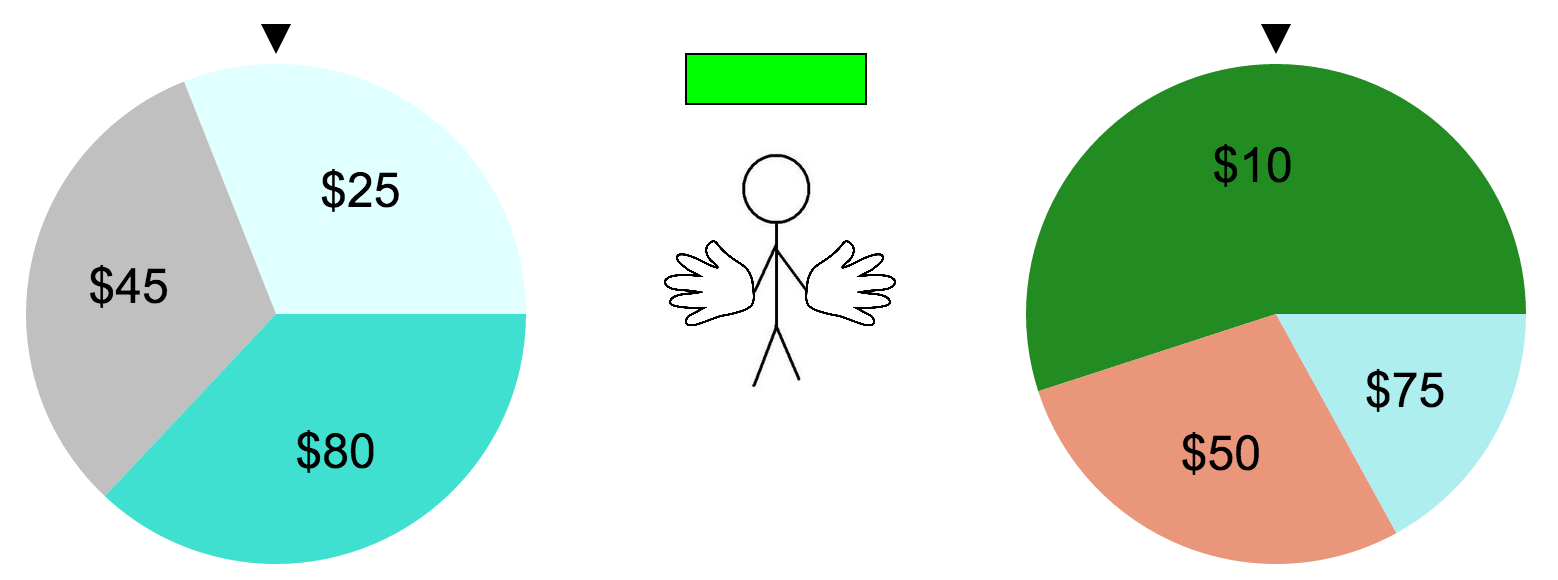
\includegraphics[width=\columnwidth]{images/paradigmFig.png}
\caption{Screenshot of Experiment 1. Participants saw a character spin two wheels sequentially.}
\label{ParadigmFig}
\end{figure}

Participants played the role of observers and watched characters play a simple gambling game, described above (Fig. \ref{ParadigmFig}). On each trial, each character played 2 wheels, spun consecutively. The order of the wheels, left-then-right or right-then-left, was randomized across trials. After the outcome of each wheel, participants gave ratings of how the character feels, using six different Likert scales, for each of six different emotions: happiness, sadness, contentment, disappointment, relief and regret (Fig. \ref{ParadigmFig2}). After they gave ratings to the second wheel, they then gave an overall judgment of the character's emotions. Thus, on each trial, participants made three emotion attributions: one after the result of each wheel, and one overall. Each participant completed 5 trials.


%We pre-generated a total of 50 scenarios, where each scenario corresponds to a particular outcome on a particular wheel. On each trial, the experimental program selected the scenario (the particular outcome to be won) randomly from the total set of 50 scenarios, and not proportional to the sector size within a wheel . This was a design choice to ensure that small sectors (with low notational probability) were equally represented in the data. This fact was not obvious to the participants, and we assume that participants treated the wheel as being fairly spun. The exact position within the sector where the spinner lands�for example, whether the spinner lands in the center of the sector, or near the edge of the sector, as in the example shown in Figure 3�was drawn from a uniform distribution.



\begin{figure}[htb!]
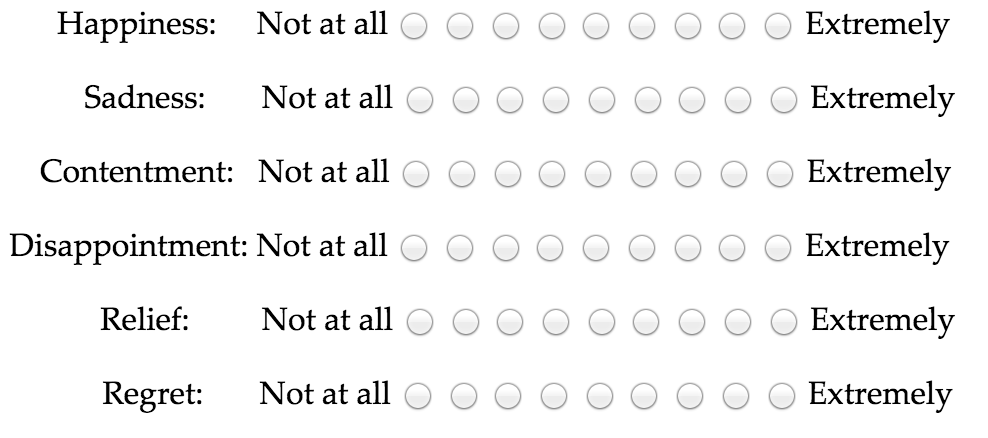
\includegraphics[width=\columnwidth]{images/paradigmFig2.png}
\caption{Dependent measures for Experiments 1 and 2. Participants gave emotion attributions along six emotions, 1) following each wheel, and 2) overall.}
\label{ParadigmFig2}
\end{figure}

\subsubsection{Results.}

First, we modeled each of the relational attributions using features from both events. That is, we fit the crosstalk model for both events $X$ and $Y$:
\begin{align} \label{RelationalEmotionModel}
E_R(A; (X,Y)) &= b_0 + b_1 \text{win}(X) + b_2 \text{PE}(X) + b_3 \text{absPE}(X) \\
&\qquad +  b_4 \text{win}(Y) + b_5 \text{PE}(Y) + b_6 \text{absPE}(Y) + \epsilon  \nonumber
\end{align}

Hypothesis \ref{Hypothesis:NoCrossTalk} (``Independence") would predict that when Eqn. \ref{RelationalEmotionModel} is used to predict $E_R(A,X)$, the coefficients $\{b_4,b_5,b_6\}$ should be close to 0 (and conversely, the coefficients $\{b_1,b_2,b_3\}$ should be 0 when predicting $E_R(A,Y)$). In contrast, Hypothesis \ref{Hypothesis:CrossTalk} (``No Independence") would predict that those coefficients will be non-zero.

The results of fitting Eqn. \ref{RelationalEmotionModel} (i.e., \{$b_1,\ldots, b_6$\}), with random effects by subject and wheels, are presented in Fig. \ref{Expt1Results1}. We note two major results. First, there seems to be no evidence for any dependence across the two attributions. Across all the emotions and collapsed across both events $X$ and $Y$, the features of the other event do not affect the judgments of the considered event ($\chi^2(3)=1.36, p=0.72$). This result supports the independence hypothesis, or Hypothesis \ref{Hypothesis:NoCrossTalk}. Observers are able to make independent judgments about emotions following two events X, Y that occur to an agent.

Second, making two relational attributions qualitatively changes the features considered during attribution. In particular, there does not seem to be evidence for any dependency on absPE when considering all the emotions ($\chi^2(1)=1.13, p=0.29$), although it still matters for Sadness ($\chi^2(1)=5.29, p=0.02$) and marginally for Disappointment ($\chi^2(1)=3.10, p=0.08$). Participants seem to exhibit no loss aversion, except for Sadness\footnote{In Ong, Zaki, and Goodman (under review), we find significant effects of loss aversion across all emotions, even the positive emotions.}. Thus, even though $E_R(A,\mathscr{F}(X))$ does not depend on $\mathscr{F}(Y)$, the mere presence of event $Y$ changes $\mathscr{F}(X)$. In particular, the fact that the agent will experience a second event seems to remove the effects of loss aversion. One argument could be from amortizing losses: even if the agent gets a bad outcome on event $X$, he still has a chance to make it up and get a good outcome on event $Y$, and so the expectation of future non-losses might reduce loss aversion in the present. If the probability of a bad outcome is $p$, the probability of two bad outcomes is $p^2$. Similarly, this argument works the other way: if the agent receives a bad outcome on the second event $Y$, odds are he had received a good outcome on the past event $X$, and so that might remove loss aversion on the present event $Y$.




\begin{figure}[htb!]
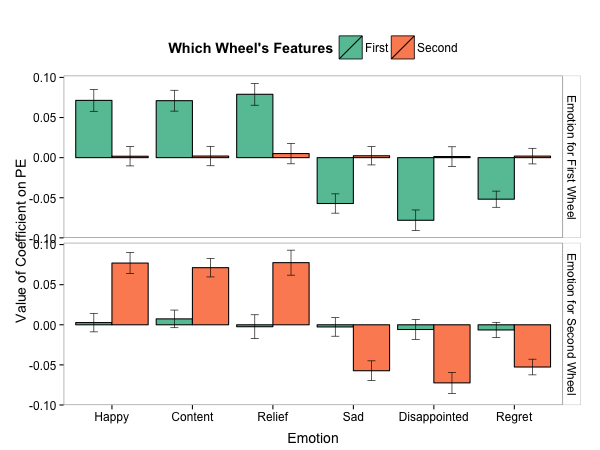
\includegraphics[width=\columnwidth]{images/Expt1Coefficients.png}
%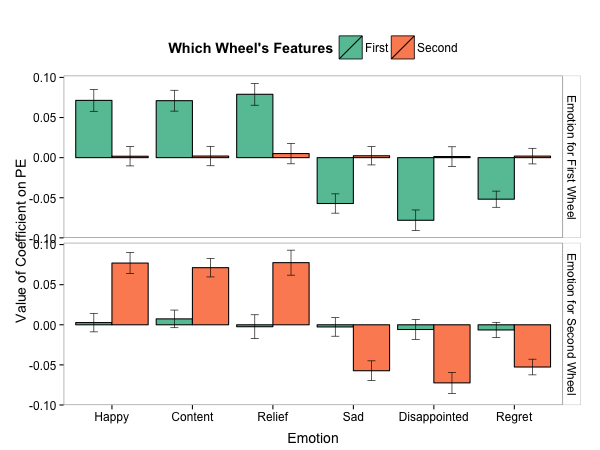
\includegraphics[width=\textwidth]{images/Expt1Coefficients.png}
\caption{ Experiment 1 Results. Weights on the different features in $\mathscr{F}$: win, PE, and absPE, along with 95\% confidence intervals. Coefficients belonging to the first wheel are in green; those belonging to the second wheel are in orange. The top row of panels indicates emotion attribution after the first wheel, while the bottom row, after the second wheel. }
\label{Expt1Results1}
\end{figure}

Next, we proceeded to model the overall emotion as a linear combination of the two relational attributions, i.e., 
\begin{align} \label{OverallEmotionModel}
E_S(A) = b_0 + b_1 E_R(A,X) + b_2 E_R(A,Y) + \epsilon
\end{align}
Hypothesis \ref{Hypothesis:SimpleAverage} would predict that the weights on the two relational attributions would be similar ($b_1 = b_2$), while Hypothesis \ref{Hypothesis:RecencyWeighted} would predict that the weight on the temporally-later (more recent) attribution would carry more weight ($b_2 > b_1$). The results of the model in Eqn. \ref{OverallEmotionModel}, with additional random effects by subject and wheels, are shown in Figure \ref{Expt1Results2}. The coefficients on the second emotion were consistently higher than those on the first emotion, across all six emotions measured ($\chi^2(6)=278.04, p\ll.001$). The ratio $b_2/b_1$ ranged from 1.42 (for Content) to 2.21 (for Regret), with an average of 1.68; thus, on average the second relational emotion attributed was weighted almost 70\% more than the first relational emotion attributed. These results support Hypothesis \ref{Hypothesis:RecencyWeighted}: observers seem to be weighing recent events more than less-recent events.

\begin{figure}[htb!]
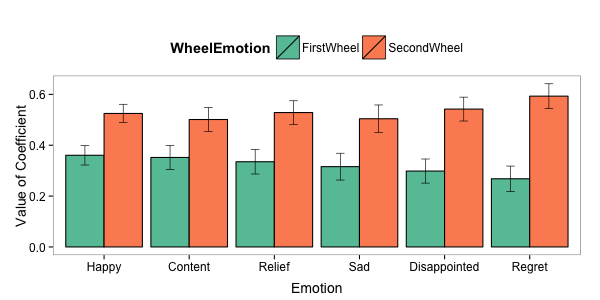
\includegraphics[width=\columnwidth]{images/Expt1OverallEmotion.png}
\caption{ Experiment 1 Results. Weights on the relational attributions in predicting the overall attribution, with 95\% confidence intervals. The second relational emotion is consistently weighted on average 70\% more than the first relational emotion.}
\label{Expt1Results2}
\end{figure}







\subsection{Experiment 2}

In Experiment 1, participants saw the two events X and Y in the temporal order in which they occurred (event X occurred, then event Y; participants rated event X, then event Y). The results of Experiment 1 could be due either to the fact that 1) participants were sensitive to the fact that agents weight more recent events more strongly (\textit{agent-recency}), or 2) participants were more affected by the order of judgments they gave (\textit{observer-recency}), or both. Experiment 2 sought to investigate these two recency effects by dissociating the temporal order of the events from the evidence order presented to participants.

\subsubsection{Participants.} 

We recruited 150 participants through Amazon's Mechanical Turk and randomly assigned them into a \textit{Congruent} (N=79) or an \textit{Incongruent} (N=71) condition.

\subsubsection{Procedures.} 

\begin{figure}[htb!]
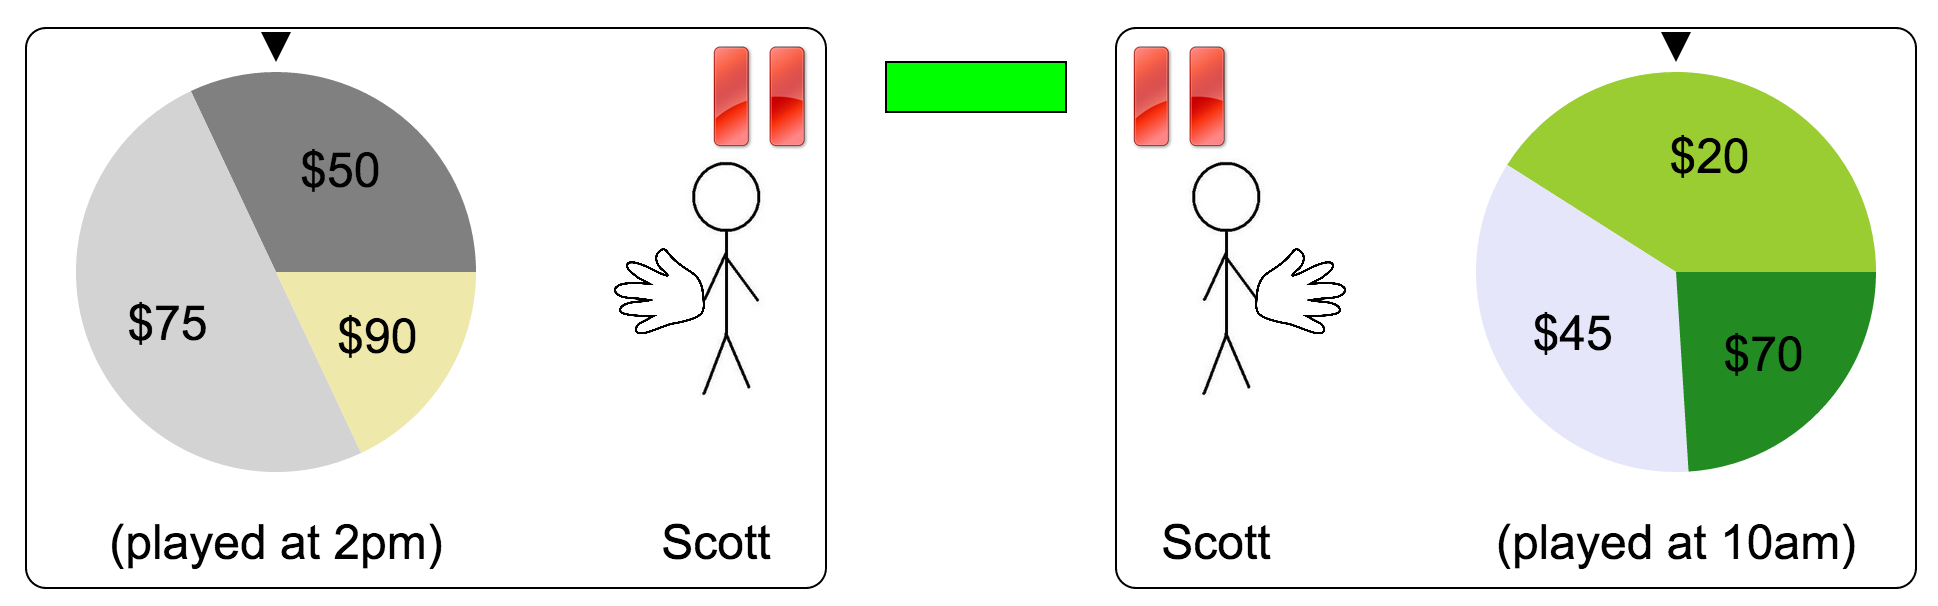
\includegraphics[width=\columnwidth]{images/paradigmFig3.png}
\caption{Screenshot of Experiment 2. The two wheels were ostensibly spun at different times, and the order in which the wheels were presented differed across conditions.}
\label{ParadigmFig3}
\end{figure}


The procedure is similar to Experiment 1, except that the stick figure character played one wheel at 10am (the \textit{temporally-earlier} wheel), and one wheel at 2pm (the \textit{temporally-later} wheel). The two wheel spins were presented as TV recordings (Fig. \ref{ParadigmFig3}). In the \textit{Congruent} condition, participants first saw the character spin the 10am wheel, then the 2pm wheel. In the \textit{Incongruent} condition, participants first saw the 2pm wheel, then the 10am wheel. In both conditions, similar to Experiment 1, they made attributions following each wheel, and then made an overall attribution (``How does A feel overall immediately after the 2pm spin?").




\subsubsection{Results.}

In the Congruent condition, which is in essence a replication of Experiment 1 with additional timing information, both \textit{agent-recency} and \textit{observer-recency} effects, if they exist, would contribute to increased weight on the temporally-later emotion. In the Incongruent condition, we made the \textit{agent-recency} and \textit{observer-recency} effects incongruent with each other. We reversed the order of presentation, asking participants to first attribute a temporally-later emotion (``2pm"), before attributing a temporally-early emotion (``10am"). If participants were only sensitive to \textit{agent-recency}, then the pattern of results should be identical to the Congruent condition: i.e., participants would still weight the 2pm emotion more than the 10am emotion. If participants were susceptible to \textit{observer-recency} effects, then the pattern should flip completely, with participants weighting the 10am emotion (the attribution they had made more recently) more than the 2pm emotion.


\subsubsection{Evidence for both agent-recency and observer-recency.}

\begin{figure}[htb!]
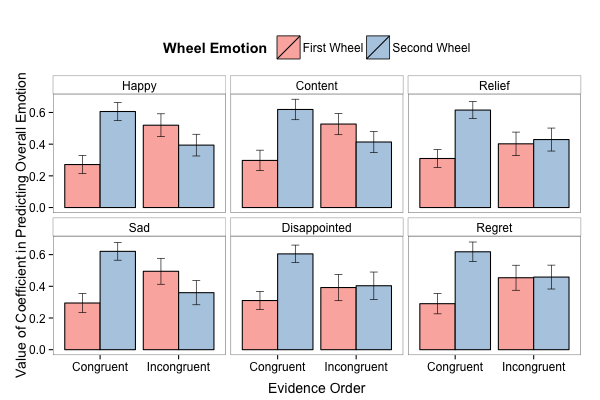
\includegraphics[width=\columnwidth]{images/Expt2OverallEmotion.png}
\caption{ Experiment 2 Results. Weights on the relational attributions in predicting the overall attribution, with 95\% confidence intervals. Temporally-earlier relational attributions (``10am emotions") are in green, while temporally-later relational attributions (``2pm emotions") are in orange.}
\label{Expt2Results2}
\end{figure}

The results are shown in Fig. \ref{Expt2Results2}. For the Congruent condition, we replicated the results of Experiment 1: there is a stronger weighting of the temporally-later emotion as compared to the temporally-earlier emotion ($\chi^2(6)=240.88, p\ll.001$). The ratio $b_2/b_1$ (Eqn. \ref{OverallEmotionModel}) ranged from 1.95 for Disappointment to  2.23 for Happiness, with an average of 2.08. This means that on average, participants more than doubled the weight on the temporally-later emotion compared to the temporally-earlier emotion. Note that the effect size here is slightly larger than that in Experiment 1, but this is consistent with the different presented time-frames---In Experiment 1, the wheels were spun consecutively, while there was an ostensible 4 hour delay between the two wheels in Experiment 2.

In the Incongruent condition, we observe an interesting interaction. For Happy, Content, and Sad, the temporally-later emotion (the first attribution participants gave) is still weighted more than the temporally-earlier emotion (the second attribution participants gave), although the effect size is lower in magnitude than the Congruent condition ($b_2/b_1 = 1.32, 1.27, 1.38$ respectively). The difference in weighting disappears in Relief, Disappointed, and Regret ($b_2/b_1 = 0.94, 0.97, 0.99$ respectively). Across all the emotions, the temporally-later emotion is still weighted more than the temporally-earlier emotion (mean $b_2/b_1$=1.14, $\chi^2(6)=17.64, p=.007$). This patten of results supports the existence of both agent-recency and observer-recency effects, with the former perhaps a little stronger than the latter.



%When human observers attribute emotions to others, they are often doing so with respect to 
%
%
%
%Social life constantly requires us to decipher information about others into inferences about their emotional states: for example, we have to reason about what makes our romantic partners happy (a surprise gift?) or angry (not doing one's chores?), and what they would do in those emotional states, in order to plan our upcoming interactions. Such \textit{affective cognition}, or our ability to reason about others' emotions, scaffolds everything from cooperation to the maintenance of social relationships. Affective cognition lies in the intersection of two foundational social cognitive topics, Theory of Mind (ToM; the ability to reason about others' mental states) and Empathy (the ability to feel and understand others' emotions). Although the past decade has seen much progress in understanding ToM and empathy using neuroscience \cite{Koster-Hale2013, Zaki2012}, developmental \cite{Meltzoff2011}, and computational \cite{Baker2009, Goodman2013} approaches, somewhat less attention has been paid specifically to affective cognition and some of its foundational cognitive questions. How do we represent (cognitively and neurally) others' emotional states? How do we reason with those representations? How do we make predictions and inferences about others' future actions or desires based on their emotions? Finally, how does affective cognition shift across development? The aim of the symposium is to answer these, and other relevant questions, at the forefront of this field.
%
%
%Humans are extremely skilled at reasoning about others� emotions; this ability is crucially important to forming and maintaining social relationships. Yet despite its importance, few formal or quantitative theories have successfully described how affective cognition operates. Here we address this gap by constructing a computational model, drawing on tools from Bayesian statistics. We use a simple gambling paradigm to quantitatively test this model, finding that emotion judgments are well explained in terms of a low-dimensional representation based on value-related computations. Further, we demonstrate that emotion inferences across multiple situations are tightly predicted by Bayes� rule. Our results speak to a deep structural relationship between emotions and cognitive inference, and suggest wide-ranging applications to basic psychological theory and psychiatry.



\section{Discussion}

\section{Acknowledgments}

This work was supported in part by an A*STAR National Science Scholarship to DCO and by a James S. McDonnell Foundation Scholar Award to NDG.


\bibliographystyle{apacite}

\setlength{\bibleftmargin}{.125in}
\setlength{\bibindent}{-\bibleftmargin}

\bibliography{relationalToE}


\end{document}
